\documentclass[crop,tikz]{standalone}
\usepackage{amsmath,amssymb}
\usepackage{pgfplots}

\definecolor{cliquecolor}{HTML}{457B9D}
\newcommand{\cliquecolor}{cliquecolor!75!blue}
\definecolor{cyclecolor}{HTML}{CC5800}
\newcommand{\cyclecolor}{cyclecolor!75!red}

\begin{document}
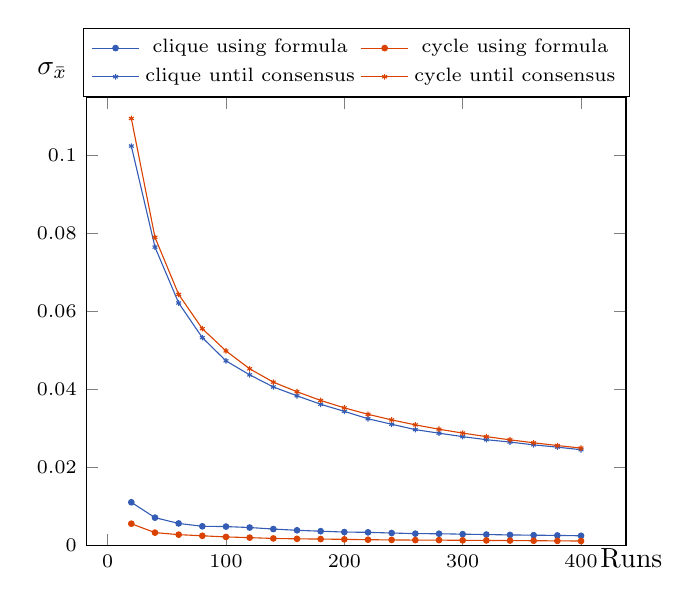
\begin{tikzpicture}
  \pgfplotsset{yticklabel style={/pgf/number format/fixed, /pgf/number format/precision=3}, scaled y ticks=false}
  \pgfplotsset{every axis legend/.append style={at={(0.5,1)},anchor=south}} %%% To put legend outside the box
\begin{axis}[legend columns=2, %%% Legends horizontally
        %axis equal image=true,unit vector ratio=9 1,width=1.1\columnwidth, %%% size of box
        ymin=0,
        ymax=0.115,
        every tick label/.append style={font=\scriptsize},legend style={font=\scriptsize}, %%% size of legends
        xlabel=Runs, ylabel=$\sigma_{\bar{x}}$, %%% axis labels
        every axis y label/.style={at={(ticklabel cs:1.02)},anchor=south west}, %%%% position of y-axis legend
        every axis x label/.style={at={(ticklabel cs:1.01)},anchor=south}, %%%% position of y-axis legend
        ]
    %\draw[help lines] (axis cs:0,1) -- (axis cs:3,1);
\addplot[color=\cliquecolor,mark=*,mark size=1pt] coordinates {
  (20, 0.011092)
  (40, 0.007149)
  (60, 0.005665)
  (80, 0.004934)
  (100, 0.004862)
  (120, 0.004613)
  (140, 0.004225)
  (160, 0.003906)
  (180, 0.003671)
  (200, 0.003453)
  (220, 0.003380)
  (240, 0.003210)
  (260, 0.003048)
  (280, 0.003022)
  (300, 0.002908)
  (320, 0.002815)
  (340, 0.002716)
  (360, 0.002649)
  (380, 0.002591)
  (400, 0.002498)
};
\addplot[color=\cyclecolor,mark=*,mark size=1pt] coordinates {
  (20, 0.005595)
  (40, 0.003308)
  (60, 0.002790)
  (80, 0.002496)
  (100, 0.002202)
  (120, 0.002021)
  (140, 0.001812)
  (160, 0.001712)
  (180, 0.001658)
  (200, 0.001579)
  (220, 0.001489)
  (240, 0.001439)
  (260, 0.001390)
  (280, 0.001383)
  (300, 0.001333)
  (320, 0.001303)
  (340, 0.001268)
  (360, 0.001229)
  (380, 0.001195)
  (400, 0.001155)
};
\addplot[color=\cliquecolor,mark=asterisk,mark size=1pt] coordinates {
  (20, 0.102470)
  (40, 0.076547)
  (60, 0.062212)
  (80, 0.053327)
  (100, 0.047371)
  (120, 0.043773)
  (140, 0.040671)
  (160, 0.038397)
  (180, 0.036239)
  (200, 0.034407)
  (220, 0.032517)
  (240, 0.031106)
  (260, 0.029726)
  (280, 0.028818)
  (300, 0.027926)
  (320, 0.027151)
  (340, 0.026535)
  (360, 0.025820)
  (380, 0.025235)
  (400, 0.024568)
};
\addplot[color=\cyclecolor,mark=asterisk,mark size=1pt] coordinates {
  (20, 0.109545)
  (40, 0.079057)
  (60, 0.064406)
  (80, 0.055621)
  (100, 0.049910)
  (120, 0.045332)
  (140, 0.041907)
  (160, 0.039451)
  (180, 0.037210)
  (200, 0.035311)
  (220, 0.033660)
  (240, 0.032220)
  (260, 0.030950)
  (280, 0.029832)
  (300, 0.028844)
  (320, 0.027931)
  (340, 0.027109)
  (360, 0.026351)
  (380, 0.025648)
  (400, 0.024995)
};
\legend{clique using formula, cycle using formula, clique until consensus, cycle until consensus}
\end{axis}
\end{tikzpicture}
\end{document}
